% Sandia National Laboratories is a multimission laboratory managed and
% operated by National Technology & Engineering Solutions of Sandia, LLC, a
% wholly owned subsidiary of Honeywell International Inc., for the U.S.
% Department of Energy’s National Nuclear Security Administration under
% contract DE-NA0003525.

% Copyright 2002-2024 National Technology & Engineering Solutions of Sandia,
% LLC (NTESS).


%%
%% Table describing the flatx, flaty parameters.
%%

\newenvironment{FlatTable}[1]
               {\renewcommand{\arraystretch}{1.5}
                 \newcommand{\category}[1]{\multicolumn{4}{c}{\smallskip\color{XyceDarkBlue}\em\bfseries ##1}}
                 \begin{longtable}{>{\ttfamily\small}m{1in}<{\normalfont}>{\raggedright\small}m{3in}>{\raggedright\let\\\tabularnewline\small}m{1in}}
                   \caption{#1} \\ \hline}
               {\end{longtable}}

%% ERK: Note:  I made each row of the table actually be two rows, because the 
%% graphical cross section picture, which is coming from a jpg file, was 
%% tending to overwrite the lines of the table.  In particular, it was 
%% overwriting the line immediately above it.  It did this for every 
%% (length, width) value that I tried.
%%
\begin{FlatTable}{Description of the flatx, flaty doping parameters\label{flatxy_table}}
    \rowcolor{XyceDarkBlue}
    \color{white}\normalfont\bf Flatx or Flaty view  &
    \color{white}\bf Description &
    \color{white}\bf 1D Cross Section \endhead

   0  & Gaussian on both sides of the peak (\texttt{xloc}) location. & {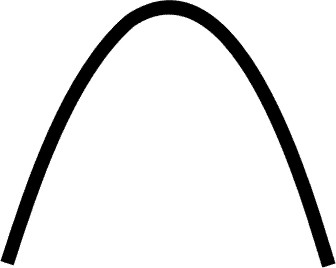
\includegraphics[width=0.300in,height= 0.300in]{flatxy1}} \\ \hline
  +1  & Gaussian if \texttt{x>xloc}, flat (constant at the peak value) if \texttt{x<xloc}. & {
\includegraphics[width=0.300in,height= 0.300in]{flatxy2}} \\ \hline
  -1  & Gaussian if \texttt{x<xloc}, flat (constant at the peak value) if \texttt{x>xloc}. & {
\includegraphics[width=0.300in,height= 0.300in]{flatxy3}} \\ \hline
\end{FlatTable}

